\documentclass[10pt]{article}
\usepackage[a4paper,margin=1in]{geometry}
\usepackage[T1]{fontenc}
\usepackage{amsmath,amssymb,amsthm,booktabs,graphicx}
\newcommand{\citep}[1]{\cite{#1}}
\usepackage[hidelinks]{hyperref}
\newtheorem{proposition}{Proposition}
\newtheorem{remark}{Remark}
\newcommand{\E}{\mathbb{E}}
\newcommand{\Var}{\operatorname{Var}}
\newcommand{\Cov}{\operatorname{Cov}}
\title{Auditable Neural Martingale Control Variates\\for Basket Option Pricing}
\author{Siddhartha G.\\\small Independent research draft}
\date{October 26, 2026}
\begin{document}
\maketitle

\begin{abstract}
Small Monte Carlo standard errors do not establish accurate option prices when
a learned control variate is centered at an incorrect expectation. We reconstruct
a neural PDE pricing project whose saved one-dimensional hybrid estimate is
8.95\% below its analytical reference despite a reported standard error of
$4.32\times10^{-7}$. We identify the centering failure, separate inherited
artifacts from new measurements, and implement predictable neural martingale
controls with independent pilot fitting and explicit reference uncertainty.
The resulting study compares smooth Deep Galerkin and multilayer-perceptron
surrogates with plain Monte Carlo, antithetic sampling, geometric-basket controls,
and scrambled Sobol integration. Analytical calibration isolates the effects of
control resolution and inaccurate gradients from approximation bias. Our
contribution is an auditable implementation and evaluation protocol, not a new
martingale identity or an assertion of state-of-the-art performance. The
finite-budget results include 18 freshly trained models and 1,872 pricing
estimates. At the central scenarios, DGM controls reduce estimated standard
errors by approximately 4.5--5.4 times relative to plain Monte Carlo, but cheap
geometric controls are substantially faster. The study therefore supports
estimator validity, not a claim of practical neural superiority.
\end{abstract}

\section{Introduction}
Neural PDE solvers offer mesh-free function approximations in settings where
tensor-product spatial grids are impractical. A learned price, however, remains
an approximation. Automatic differentiation returns derivatives of that
approximation, not necessarily accurate financial sensitivities. Monte Carlo
control variates offer a complementary use of a learned model: preserve the
target expectation while altering sampling variance. This separation is useful
only when the control's expectation is genuinely known.

We investigate this distinction in an inherited basket-pricing project. Its
near-terminal network predictions were highly correlated with realized payoffs,
but were centered at an unverified time-zero network prediction. A small residual
sample variance then coexisted with a substantial price error. Other inherited
tables mixed relative $L^2$ and mean relative errors, and some aggregate entries
were rescaled from different sampling budgets. These findings motivate a
reconstruction rather than cosmetic revision of the original claims.

Our contributions are threefold: (i) an explicit diagnostic counterexample and
source-level audit; (ii) a self-contained smooth PDE implementation and
independently piloted martingale estimator; and (iii) an immutable, multi-seed
screening study with strong classical comparators, analytical calibration, and
cost accounting. We do not equate unbiasedness, variance reduction, computational
efficiency, novelty, and industrial readiness: each requires separate evidence.

\section{Related work and scope}
The Deep Galerkin Method (DGM) of Sirignano and Spiliopoulos
\citep{sirignano2018} trains a neural approximation using differential-equation
residuals and condition losses. We use its gated architecture as a baseline,
not as a new architectural contribution. Deep BSDE methods
\citep{han2018} offer a probabilistic alternative; we discuss but do not claim
to reproduce them in the new experiments.

Most directly, Sabate Vidales, \v{S}i\v{s}ka and Szpruch
\citep{vidales2022} combine approximate neural gradients with martingale
controls, including high-dimensional experiments. Hinds and Tretyakov
\citep{hinds2023} study neural variance reduction for Brownian and
L\'evy-driven SDEs, including direct variance-based learning. Consequently,
reframing a neural PDE solution as a control variate is not itself new.
Our narrower contribution is a reproducible analysis of failure modes and
the incremental value of neural controls after a cheap analytic control.
Neither the classical projection formulas below nor conditional unbiasedness
is asserted as a new theorem.

\section{Problem and failure diagnosis}
Let $x_i=\log(S_i/K)$ and
\begin{equation}
 dx_t=\mu\,dt+B\,dW_t,\qquad
 \mu_i=r-\tfrac12\sigma_i^2,\quad BB^\top=A,
 \quad A_{ij}=\rho_{ij}\sigma_i\sigma_j.
\end{equation}
The arithmetic basket payoff is
$\phi(x)=K(d^{-1}\sum_i e^{x_i}-1)^+$ and the target price is
$v=\E[Y]$, where $Y=e^{-rT}\phi(x_T)$.
The log-coordinate pricing operator is
\begin{equation}
 \mathcal L u=\partial_tu+\mu^\top\nabla_xu+
 \tfrac12\operatorname{tr}(A\nabla_x^2u)-ru.
\end{equation}

\subsection{Why terminal correlation is insufficient}
For a control $C$ centered at a proposed mean $m$ and a fixed coefficient $b$,
\begin{equation}\label{eq:wrongmean}
 \E[Y-b(C-m)]-v=-b(\E[C]-m).
\end{equation}
High correlation says nothing about the right-hand side. In particular, take
$C=\phi(x_T)$, $m=v$, and $b=e^{-rT}$. Then every adjusted observation is
exactly $e^{-rT}v$: the sample variance vanishes, but the estimator is biased
unless $rT=0$ or $v=0$. Even using the exact terminal payoff does not repair the
incorrect mean.

For a sufficiently regular approximate solution $u$, It\^o's formula gives
\begin{equation}
 \E[e^{-rT}u(T,x_T)]
 =u(0,x_0)+\E\!\int_0^T e^{-rt}\mathcal L u(t,x_t)\,dt.
\end{equation}
Thus even after correcting discounting, the initial value of an approximate PDE
solution is not generally the expectation of its discounted terminal value.

\paragraph{Inherited evidence, not a new experiment.}
The saved 1D hybrid price is $0.095156352459$. The exact
Black--Scholes value at $S_0=K=1$, $r=0.05$, $\sigma=0.2$, $T=1$ is
$0.104505835722$. Their difference is approximately 21,638 reported hybrid
standard errors. This calculation is independently reproduced by the audit
command. No legacy performance value is imported into the new experiment tables.

\subsection{Other corrected sources of invalid inference}
The reconstruction removes a payoff lifting that switched between smooth and
kinked functions at train/evaluation time; a zero-value boundary penalty that
was false on multidimensional basket faces; and a stochastic trace estimate
whose square optimized $R^2+\Var(\widehat R)$ rather than $R^2$.
It also replaces individual-path antithetic uncertainty by pair-level
uncertainty and eliminates test-based checkpoint selection. The full audit
provides original file paths and distinguishes source inspection from reruns.

\section{Corrected estimator and implementation}
\subsection{Predictable neural controls}
Fix a model $u_\theta$ trained independently of evaluation paths. For a grid
$0=t_0<\cdots<t_M=T$, define
\begin{equation}\label{eq:integral}
 C_\theta=\sum_{k=0}^{M-1}e^{-rt_k}
 \nabla_xu_\theta(t_k,x_{t_k})^\top B\Delta W_k.
\end{equation}
The gradient is evaluated before the new Brownian increment. We use exact
Gaussian log-price transitions; control discretization therefore changes
variance but does not introduce payoff discretization bias in this model.

\begin{proposition}[Conditional unbiasedness]
Let $\mathcal H$ contain training and independent pilot information. Suppose the
frozen integrands in \eqref{eq:integral} are predictable and square integrable
conditional on $\mathcal H$. Let $G$ be another integrable control with
$\E[G\mid\mathcal H]=0$, and let $\widehat b$ be a finite,
$\mathcal H$-measurable coefficient vector. For fresh independent paths,
\begin{equation}
 \widehat v=N^{-1}\sum_{n=1}^N
 \left(Y_n-\widehat b_1G_n-\widehat b_2C_{\theta,n}\right)
\end{equation}
satisfies $\E[\widehat v\mid\mathcal H]=v$. Unconditional unbiasedness follows
when the adjusted observations are integrable.
\end{proposition}
\begin{proof}
Each summand of $C_\theta$ has zero conditional expectation by independence and
zero mean of the fresh Brownian increment. Apply the tower property, the
known zero mean of $G$, and measurability of $\widehat b$.
\end{proof}

This result does not guarantee variance reduction. For the exact price function
and continuous-time integrand $h^*$, the martingale representation yields
$Y-v=\int_0^T(h_t^*)^\top dW_t$. For any admissible stepwise approximation
$h$, It\^o isometry gives
\begin{equation}
 \Var\left(Y-\int_0^Th_t^\top dW_t\right)
 =\E\int_0^T\|h_t^*-h_t\|^2dt.
\end{equation}
This identity explains why price accuracy and useful control gradients are
related but distinct, and why deliberately bad gradients can increase variance.

\subsection{Geometric control and incremental neural value}
For $\phi_g(x)=K(e^{\bar x}-1)^+$, use
$G=e^{-rT}\phi_g(x_T)-v_g$, where $v_g$ is an exact lognormal expectation.
Writing $m=\bar x_0+\bar\mu T$, $q=T d^{-2}\mathbf1^\top A\mathbf1$,
\begin{equation}
 v_g=Ke^{-rT}\left[e^{m+q/2}\Phi((m+q)/\sqrt q)
                          -\Phi(m/\sqrt q)\right],
\end{equation}
with the deterministic limit used when $q=0$.

With population covariance $\Sigma_C$ and $c=\Cov(C,Y)$, optimal linear
coefficients are $b^*=\Sigma_C^{\dagger}c$. To interpret adding a neural control,
residualize it against $G$: $\widetilde C=C_\theta-
\Cov(C_\theta,G)G/\Var(G)$. The population variance reduction beyond optimal
geometric control is
\begin{equation}\label{eq:incremental}
 \frac{\Cov(Y,\widetilde C)^2}{\Var(\widetilde C)},
\end{equation}
when the denominator is positive. A neural control redundant with $G$ adds no
population benefit. Independent pilot OLS approximates this projection using
centered, standardized columns and an SVD. Pilot means are not used as evaluation
centers. Finite-pilot estimation can worsen variance, so monotonic improvement
is not claimed. The one-dimensional arithmetic and geometric payoffs coincide;
their roundoff-level residual is an analytic baseline, not a neural achievement.

\subsection{Smooth training and numerical safeguards}
We train raw tanh DGM and MLP outputs with
\begin{equation}
 J(\theta)=\E[|\mathcal L u_\theta|^2]
       +10\E[|u_\theta(T,x)-\phi(x)|^2].
\end{equation}
There is no hard payoff embedding or artificial boundary-face loss. Interior
collocation uses uniform time and Gaussian log prices with standard deviation
0.3. Terminal samples use the same spatial law and the exact payoff target.
All Hessian contractions are deterministic and exact under automatic
differentiation. This is a finite-budget training baseline, not a claim of
global PDE convergence. Nonfinite losses and estimator records fail explicitly.

\section{Experimental protocol}
\label{sec:protocol}
The completed protocol uses CPU float64, fixed Adam learning rate $10^{-3}$,
300 steps, batch size 64, width 32, and depth 2. Each architecture is trained
with seeds 11, 29 and 47 at dimensions 1, 5 and 10: 18 fresh models in total.
No legacy checkpoint is loaded and no test labels choose a checkpoint.
Equal width is not equal parameter count or training cost.

We fix $K=T=1$, $r=0.05$, $\sigma_i=0.2$, $\rho_{ij}=0.3$ for $i\ne j$.
Three scenario centers are $m_0\in\{0.85,1,1.15\}$; for $d>1$ spots are
$S_{0,i}=m_0\exp(\operatorname{linspace}(-0.12,0.12,d)_i)$.
These heterogeneous vectors avoid the equal-asset diagonal, but are not a
full-dimensional test distribution. Plain MC, antithetic MC, geometric control
and RQMC additionally run at dimensions 25, 50 and 100. Those extra dimensions
provide classical context only.

Each estimate uses 1024 evaluation paths; fitted controls use another 1024
independent pilot paths. Neural controls use eight time steps. RQMC uses eight
independent scrambles of 128 Sobol points. There are eight repeated evaluations
per scenario/model. Architecture comparisons share evaluation randomness where
their scenario and training-seed labels coincide. Evaluation repetitions are not
additional independent training seeds.

One-dimensional prices use an exact analytical reference. Higher-dimensional
arithmetic baskets use a separate 16-scramble, 32768-point-per-scramble RQMC
reference, with its uncertainty retained. RMSE against this reference includes
its unknown error; it is not labelled exact pricing RMSE. Sample standard errors
use independent paths, antithetic pair means, or independent scramble means as
appropriate, with sample variance and Student-$t$ interval multipliers.

For calibration, geometric payoffs have exact prices and analytical gradients.
We test grids 4, 16 and 64 in dimensions 1, 5 and 10 with 40 replications per
setting. Additional gradient scales $-1,0,0.5,2$ at eight steps deliberately
degrade the control. These are labelled oracle diagnostics, not learned results.
Coverage uncertainty is reported using Wilson intervals.

\paragraph{Cost and provenance.}
Evaluation, pilot and training time are recorded separately. Equal path counts
are not equal compute: neural estimates require repeated gradient evaluations.
We distinguish warm evaluation-plus-pilot time from cold-start cost including
training. Hardware-specific timings are descriptive, not deployment guarantees.
An earlier 600-step protocol was interrupted by an execution timeout. Its
partial artifacts are retained locally but excluded from every new result table.
The replacement budget was fixed before its run; it is a screening study.
Run and checkpoint hashes, actual path counts, seeds, software versions and
source fingerprints accompany the measurements.

\section{Results}
\subsection{Pricing accuracy and computational cost}
The completed main run contains 18 models, 1,872 pricing-estimate records,
54 direct surrogate prices, and 840 oracle-calibration records. Its recorded
wall time is 753 seconds; this is an execution receipt, not a cross-hardware
performance claim. Table~\ref{tab:performance} reports central scenarios.
All three moneyness scenarios, individual repetitions and training-seed
dispersion are retained in machine-readable artifacts.

\begin{table}[p]
\centering\small
% Generated from immutable raw records; do not edit.
\begin{tabular}{rllrrr}
\toprule
$d$ & Method & Arch. & RMSE & RMS SE & Warm ms \\
\midrule
1 & Antithetic & CLASSICAL & 1.42e-03 & 3.18e-03 & 4.6 \\
1 & Geometric CV & CLASSICAL & 1.20e-17 & 6.42e-18 & 4.8 \\
1 & MC & CLASSICAL & 4.03e-03 & 4.61e-03 & 0.7 \\
1 & RQMC & CLASSICAL & 3.97e-04 & 4.35e-04 & 30.8 \\
1 & Combined CV & DGM & 1.55e-17 & 8.07e-18 & 383.9 \\
1 & Neural pilot & DGM & 6.72e-04 & 9.48e-04 & 383.9 \\
1 & Combined CV & MLP & 1.58e-17 & 8.39e-18 & 88.8 \\
1 & Neural pilot & MLP & 7.70e-04 & 1.04e-03 & 88.8 \\
5 & Antithetic & CLASSICAL & 2.32e-03 & 1.89e-03 & 2.4 \\
5 & Geometric CV & CLASSICAL & 3.33e-04 & 3.24e-04 & 3.7 \\
5 & MC & CLASSICAL & 2.83e-03 & 3.18e-03 & 1.4 \\
5 & RQMC & CLASSICAL & 1.83e-04 & 1.77e-04 & 19.8 \\
5 & Combined CV & DGM & 2.17e-04 & 2.70e-04 & 377.6 \\
5 & Neural pilot & DGM & 5.11e-04 & 5.94e-04 & 377.6 \\
5 & Combined CV & MLP & 2.79e-04 & 3.00e-04 & 84.9 \\
5 & Neural pilot & MLP & 6.69e-04 & 7.17e-04 & 84.9 \\
10 & Antithetic & CLASSICAL & 4.88e-04 & 1.70e-03 & 2.0 \\
10 & Geometric CV & CLASSICAL & 1.19e-04 & 2.59e-04 & 4.5 \\
10 & MC & CLASSICAL & 2.76e-03 & 2.91e-03 & 2.0 \\
10 & RQMC & CLASSICAL & 1.67e-04 & 2.08e-04 & 37.5 \\
10 & Combined CV & DGM & 2.50e-04 & 2.31e-04 & 325.5 \\
10 & Neural pilot & DGM & 5.22e-04 & 6.47e-04 & 325.5 \\
10 & Combined CV & MLP & 2.40e-04 & 2.34e-04 & 117.2 \\
10 & Neural pilot & MLP & 7.41e-04 & 8.02e-04 & 117.2 \\
\bottomrule
\end{tabular}

\caption{Central scenario results. RMSE is measured against the independent
reference; RMS SE is the root mean square of reported sampling SEs. Warm time
includes evaluation and pilot fitting, but excludes neural training. Classical
rows aggregate eight repetitions; neural rows summarize three training seeds
with eight evaluation repetitions each. These are descriptive, unequal-compute
comparisons. The exact one-asset geometric control reaches roundoff precision.}
\label{tab:performance}
\end{table}

At $d=5$, DGM's pilot-fitted neural control has RMS SE approximately
$5.94\times10^{-4}$, compared with $3.18\times10^{-3}$ for plain MC.
The combined control reduces it further to $2.70\times10^{-4}$, versus
$3.24\times10^{-4}$ for geometric control alone. This modest incremental
variance reduction costs approximately 378\,ms per combined estimate, compared
with 3.75\,ms for geometric control. At $d=10$, the corresponding combined and
geometric RMS SEs are $2.31\times10^{-4}$ and $2.59\times10^{-4}$, with warm
costs approximately 326\,ms and 4.49\,ms. These measurements do not establish a
neural cost advantage. Training costs, recorded separately, further increase
cold-start cost.

The three-state direct-price relative $L^2$ errors in
Table~\ref{tab:direct} are materially larger than the inherited headline might
suggest. DGM is more accurate than this equal-width MLP in the short runs, but
the architectures differ in parameter count and compute, and neither has been
shown to be converged. The table is not a global price-surface norm.

\begin{table}[ht]
\centering\small
\begin{tabular}{rlrr}
\toprule
$d$ & Architecture & Mean rel. $L^2$ (\%) & Seed SD (pp) \\
\midrule
1 & DGM & 2.04 & 1.06 \\
1 & MLP & 11.81 & 6.87 \\
5 & DGM & 4.27 & 0.97 \\
5 & MLP & 15.89 & 5.31 \\
10 & DGM & 11.08 & 5.20 \\
10 & MLP & 21.53 & 1.25 \\
\bottomrule
\end{tabular}

\caption{Direct surrogate pricing over the three declared spot vectors.
Mean and sample SD are across the three training seeds; pp denotes percentage
points. No evaluation-path replication is counted as an extra training seed.}
\label{tab:direct}
\end{table}

\begin{figure}[ht]
\centering
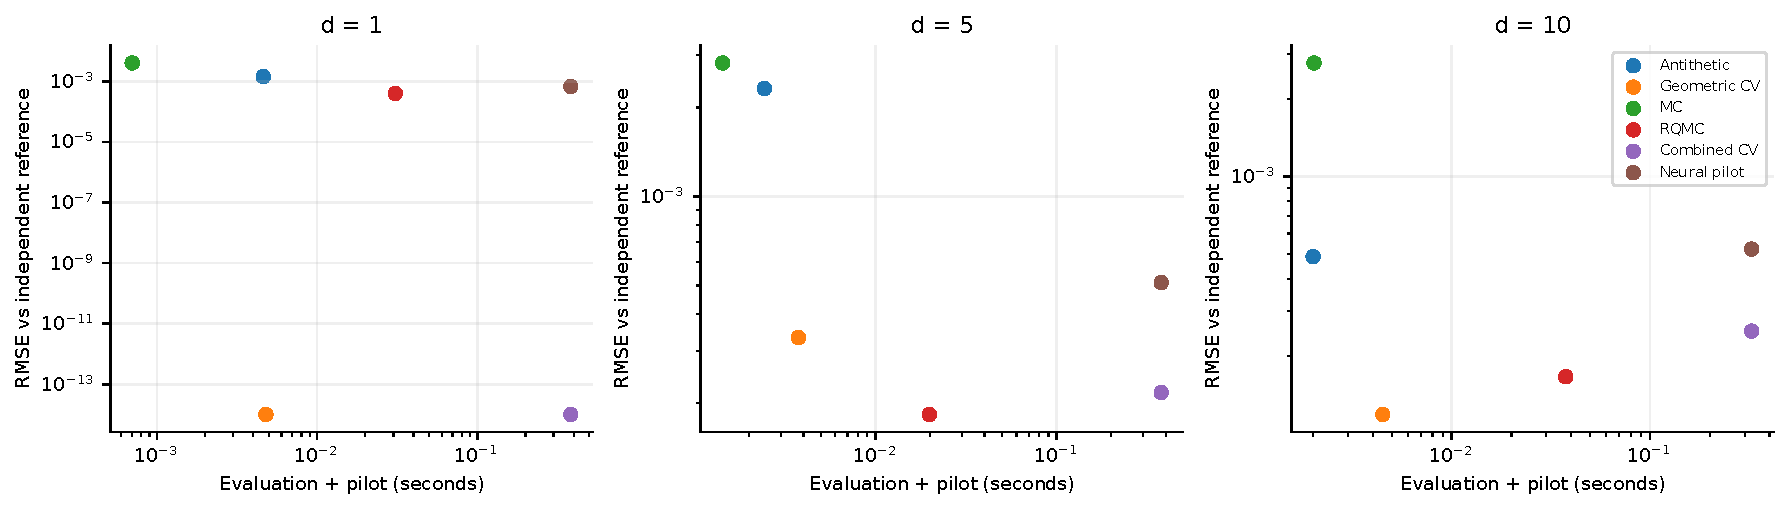
\includegraphics[width=\textwidth]{generated/cost_accuracy.pdf}
\caption{Central-scenario descriptive cost--accuracy comparison. Neural points
use DGM; MLP results remain in the table and raw data. Warm cost includes pilot
fitting. The one-dimensional roundoff-limited controls are plotted at a
$10^{-14}$ visualization floor. This is not a matched-time budget sweep.}
\label{fig:cost}
\end{figure}

\subsection{Analytical calibration and inaccurate controls}
Table~\ref{tab:calibration} separates control-grid effects from neural training.
At 64 steps, the analytical-gradient controls attain mean variance ratios
of approximately 216, 237 and 243 for dimensions 1, 5 and 10, respectively.
These are oracle results, not evidence that the learned network attains the
same accuracy. Finer control grids reduce the residual variance without
introducing bias into the exactly simulated payoff.

\begin{table}[ht]
\centering\small
\begin{tabular}{rrrrr}
\toprule
$d$ & Steps & VR factor & Coverage & Wilson 95\% interval \\
\midrule
1 & 4 & 14.8 & 1.000 & [0.912, 1.000] \\
1 & 16 & 56.0 & 0.975 & [0.871, 0.996] \\
1 & 64 & 216.1 & 0.975 & [0.871, 0.996] \\
5 & 4 & 16.6 & 0.925 & [0.801, 0.974] \\
5 & 16 & 61.3 & 0.950 & [0.835, 0.986] \\
5 & 64 & 236.9 & 0.925 & [0.801, 0.974] \\
10 & 4 & 17.3 & 0.950 & [0.835, 0.986] \\
10 & 16 & 62.4 & 0.950 & [0.835, 0.986] \\
10 & 64 & 243.4 & 0.975 & [0.871, 0.996] \\
\bottomrule
\end{tabular}

\caption{Analytical geometric-basket controls with coefficient one.
VR factor is plain-payoff sample variance divided by adjusted sample variance,
averaged over 40 replications. Coverage intervals describe uncertainty in the
observed interval coverage, not in the price.}
\label{tab:calibration}
\end{table}

The deliberately sign-reversed gradient has variance ratio about 0.256,
corresponding to roughly four times the plain-payoff variance. A zero gradient
recovers the original Monte Carlo variance. This behavior contradicts any
unconditional guarantee of variance reduction from an arbitrary network while
remaining consistent with the zero-mean-control argument. The full scale sweep
is retained, including negative results.

\begin{figure}[ht]
\centering
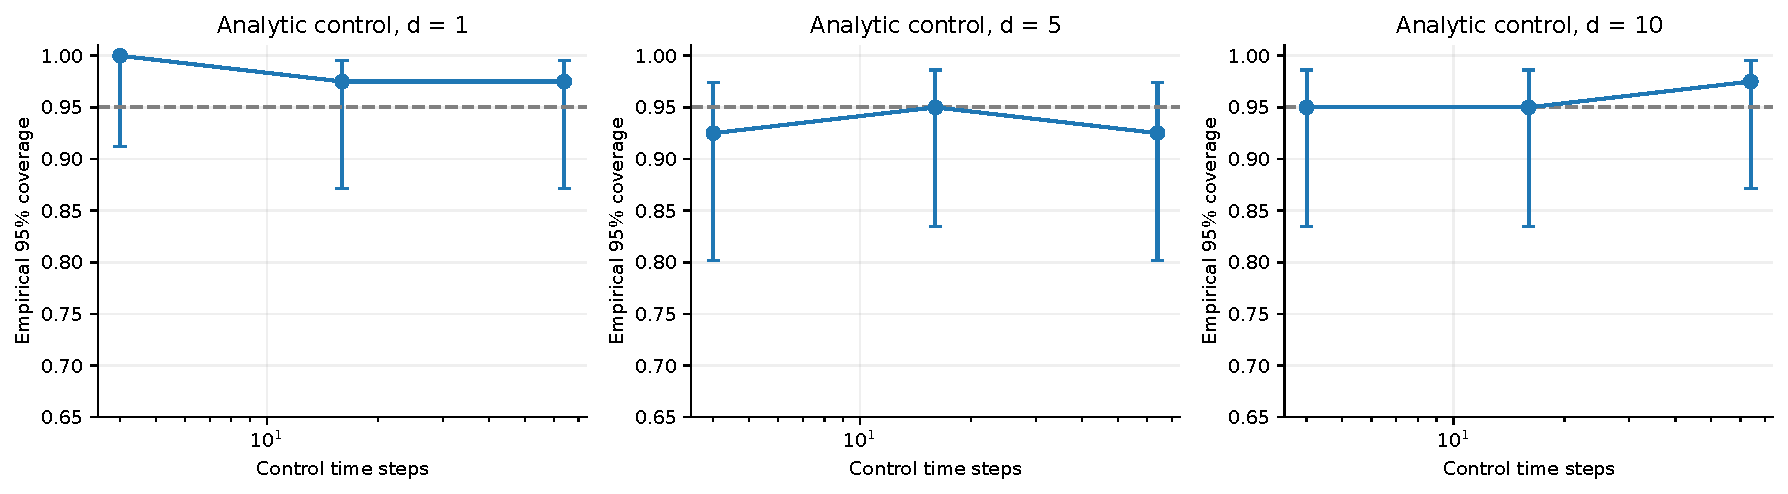
\includegraphics[width=\textwidth]{generated/coverage.pdf}
\caption{Oracle-control interval coverage with Wilson uncertainty bars and
nominal 95\% reference line. Forty repetitions per setting give wide intervals;
the plot is a diagnostic, not a proof of finite-sample calibration.}
\end{figure}

\subsection{Independent learned-control and Greek diagnostics}
An additional evaluation freezes the six one-dimensional checkpoints and runs
80 fresh repetitions per checkpoint, with 1024 pilot and 1024 evaluation paths.
Both fixed and pilot-fitted neural-only controls are evaluated, producing 960
estimate records. No additional model is selected or trained using this test.
Table~\ref{tab:learnedcoverage} reports the pilot-fitted variant. Observed
coverage ranges from 93.75\% to 100\%; one configuration covers in all 80
replications, which does not establish its true coverage. Intervals remain broad.
Each reported mean error is less than two corresponding Monte Carlo standard
errors of that mean, which is a diagnostic consistency check, not a proof that
finite-sample bias is zero.

\begin{table}[ht]
\centering\small
\begin{tabular}{lrrrr}
\toprule
Model / seed & Coverage & Wilson 95\% interval & Bias & Bias MCSE \\
\midrule
DGM / 11 & 0.9500 & [0.878, 0.980] & -9.46e-05 & 1.16e-04 \\
DGM / 29 & 0.9500 & [0.878, 0.980] & 1.63e-04 & 9.83e-05 \\
DGM / 47 & 0.9625 & [0.895, 0.987] & 1.30e-04 & 9.49e-05 \\
MLP / 11 & 0.9625 & [0.895, 0.987] & 7.95e-06 & 1.15e-04 \\
MLP / 29 & 1.0000 & [0.954, 1.000] & -1.42e-04 & 9.48e-05 \\
MLP / 47 & 0.9375 & [0.862, 0.973] & -1.25e-04 & 1.28e-04 \\
\bottomrule
\end{tabular}

\caption{Learned neural-only control coverage against exact 1D prices,
80 independent repetitions per frozen checkpoint. Bias MCSE is uncertainty of
the estimated bias across repetitions, distinct from each price estimate's SE.}
\label{tab:learnedcoverage}
\end{table}

We also evaluate price, Delta and Gamma on 101 spots from 0.6 to 1.4 at
$t=0,0.5,0.9$, for all six checkpoints: 1,818 pointwise records.
Table~\ref{tab:greeks} and Figure~\ref{fig:greeks} show that smoothness alone
does not imply accurate sensitivities. Near expiry, gamma errors are large.
Negative prices and negative gamma values occur for some checkpoints and are
recorded rather than hidden by plotting limits. These models should not be
used as validated standalone pricing or risk engines.

\begin{table}[ht]
\centering\small
\begin{tabular}{lrrrr}
\toprule
Architecture & $t$ & Price rel. $L^2$ (\%) & Delta (\%) & Gamma (\%) \\
\midrule
DGM & 0.0 & 1.89 & 5.15 & 22.31 \\
DGM & 0.5 & 2.81 & 7.14 & 33.71 \\
DGM & 0.9 & 7.28 & 19.40 & 72.74 \\
MLP & 0.0 & 15.33 & 23.07 & 62.56 \\
MLP & 0.5 & 11.22 & 16.21 & 61.60 \\
MLP & 0.9 & 8.93 & 23.79 & 84.14 \\
\bottomrule
\end{tabular}

\caption{Analytical 1D price and Greek validation over 101 spots, averaged across
three training seeds. Each column reports its own relative $L^2$ error in percent.}
\label{tab:greeks}
\end{table}

\begin{figure}[ht]
\centering
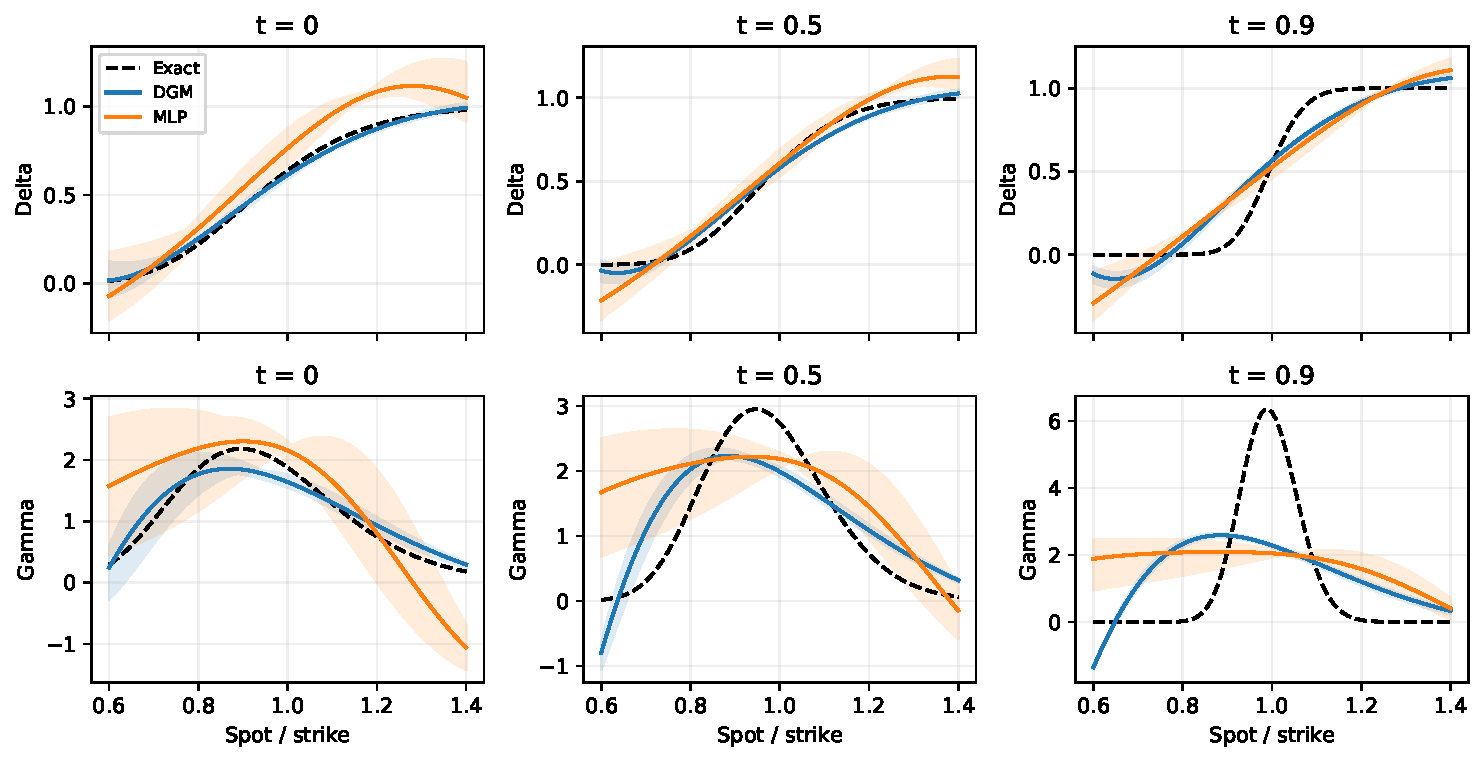
\includegraphics[width=\textwidth]{generated/greeks.pdf}
\caption{Analytical Greeks versus the mean learned Greeks; shading spans the
three seed values, not a confidence interval. Negative values are not clipped.
Near-expiry disagreement is retained as a substantive limitation.}
\label{fig:greeks}
\end{figure}

\section{Limitations and implications}
\paragraph{Validity is not novelty or optimality.}
The estimator follows established martingale-control theory. Its conditional
unbiasedness survives inaccurate frozen gradients, but neither optimal variance
nor a practical speedup follows. A credible new method must improve on strong
classical and neural variance-reduction baselines, not just plain MC.

\paragraph{Finite-budget scope.}
Three hundred training steps are insufficient to establish convergence. There
are only three training seeds and three arithmetic-basket evaluation vectors
per dimension. There is no neural scaling experiment beyond $d=10$; the
$d=25,50,100$ results are classical-only. The main pricing model has fixed
coefficients and a single payoff family. Market calibration, stochastic
volatility, jumps, early exercise and out-of-distribution robustness remain
unexamined. The analytical extension tests Greeks, but does not establish
hedging performance.

\paragraph{Statistical and computational qualifications.}
Reference Monte Carlo error is retained, not eliminated. The coverage studies
have finite replication uncertainty; the main-study RMSE comparisons are
descriptive and do not support statistical dominance claims. Timing includes
Python overhead and reflects one CPU machine with ordinary background activity,
not a dedicated benchmark host. The Sobol construction is not tuned for effective
dimension. Training amortization and matched-wall-time optimization have not
been measured. Neither a finite-budget PDE approximation nor its automatic
derivatives satisfy no-arbitrage requirements by construction.

\paragraph{A testable next contribution.}
Equation~\eqref{eq:incremental} suggests learning only the residual component
unexplained by cheap analytic controls, then using independent pilot evidence
to decide whether the extra neural cost is warranted. A convincing extension
would need finite-sample selection analysis and matched-cost comparisons with
direct integrand learning \citep{vidales2022,hinds2023}. We identify this as
future work, not an accomplished SOTA result.

\section{Conclusion}
The reconstruction demonstrates why nearly zero sample variance can be
misleading when a learned control is incorrectly centered. Predictable
martingale controls repair the estimator's expectation without requiring a
perfect PDE solution, and independent pilots avoid fitting coefficients on
final evaluation paths. Fresh experiments confirm useful neural variance
reduction but also reveal substantial computational overhead and imperfect
direct prices and Greeks. The defensible outcome is a transparent research
artifact and a sharper question about incremental neural value, not an
industry-standard pricing method or a claim of conference-level novelty.

\paragraph{Artifact availability and research integrity.}
The isolated repository contains source, tests, configurations, completed-run
manifests, checkpoint hashes, raw results and report generators. It retains a
separate audit inventory of the original research files without modifying those
files. Tables and figures are generated from hash-verified completed runs; the
interrupted run and inherited aggregate performance are excluded. All data are
synthetic. This draft retains the lead name from the inherited manuscript;
final authorship, licensing and submission venue require owner confirmation.

\bibliographystyle{plain}
\bibliography{references}
\end{document}
